\chapter{Estado del Arte}
\label{chap:estadoarte}

\drop{E}{n} el presente capítulo se describen los conceptos teóricos que
son necesarios para establecer las bases de la elaboración del \acs{PFC}. La
descripción incluye conceptos como \acf{DQ}, \acf{OD}, \acf{LOD}, Web
Semántica y Big Data. También se describe un conjunto de tecnologías que se han utilizado
para el desarrollo del proyecto. 




\section{Web Semántica}

En \cite{bernerslee2001semantic} se define la Web Semántica como una evolución o
extensión de la Web tradicional en la que la información es dada mediante
significados bien definidos, lo que facilita el procesamiento automático del
contenido y permita a las personas y a los ordenadores trabajar en cooperación. 

Este concepto ha ido evolucionando y refinándose con el paso del tiempo. En los
siguientes apartados se introduce el concepto de Web Semántica y se explicarán
sus principales características. 

\subsection{Concepto}

El \acf{W3C} en \cite{W3CSWES} define la Web Semántica como: 

\textit{Una Web extendida, dotada de mayor significado en la que cualquier
  usuario en Internet podrá encontrar respuestas a sus preguntas de forma más
  rápida y sencilla gracias a una información mejor definida. Al dotar a la Web
  de más significado y, por lo tanto, de más semántica, se pueden obtener
  soluciones a problemas habituales en la búsqueda de información gracias a la
  utilización de una infraestructura común, mediante la cual, es posible
  compartir, procesar y transferir información de forma sencilla. Esta Web
  extendida y basada en el significado, se apoya en lenguajes universales que
  resuelven los problemas ocasionados por una Web carente de semántica en la
  que, en ocasiones, el acceso a la información se convierte en una tarea
  difícil y frustrante.}

\cite{Shadbolt:2006:SWR:1155313.1155373} define a su vez la Web Semántica como
sigue: 

\textit{La Web Semántica es una Web de información procesable - información
  derivada de los datos mediante una teoría semántica para la interpretación de
  símbolos. La teoría semántica proporciona una noción de ``significado'' en la que la
  conexión lógica de términos establece la interoperabilidad entre sistemas. }

Por otro lado, \cite{HJBL} definen nuevamente la Web Semántica de la siguiente
manera: 

\textit{La Web Semántica es una extensión de la Web actual, en la que a la
  información disponible se le otorga un significado bien definido que permita a
los ordenadores y a las personas trabajar en cooperación. Está basada en la idea
de proporcionar en la Web datos bien definidos y enlazados, permitiendo que
aplicaciones heterogéneas localicen, integren, razonen y reutilicen toda la
información presente en la Web}. 

Por lo tanto se puede establecer que la Web Semántica es una extensión de la Web
en la que se dota de capacidad de anotar información semántica a los
datos de manera que proporcionen un significado. En la última definición aparece
el concepto de ``datos enlazados'' como precursor de lo que posteriormente se
considerará Linked Data (\acs{LD}), con la idea de vincular datos mediante estándares de Web
Semántica para alcanzar los siguientes objetivos: 

\begin{enumerate}
\item Reutilizar entidades ya definidas en el modelo de Web Semántica.
\item Hacer de estas entidades conceptos únicos, evitando redundancia y
  ambigüedad en los datos. 
\item Permitir la interoperabilidad semántica entre aplicaciones heterogéneas. 
\end{enumerate}

La reutilización es posible gracias al concepto de \acf{URI} utilizado para
identificar de forma unívoca, universal y expansible un espacio de nombres de
recursos de información. 

Respecto de la interoperabilidad semántica, \cite{HALPIN} explica que la
\textit{Web Semántica es la solución al problema de la integración de datos} sin
necesidad de llevar a cabo procesos de conversión, gracias a la utilización de
un modelo de representación como \acf{RDF} y utilizando \acf{XML} como fuente
sintáctica para su intercambio. 



\subsection{Terminología de Web Semántica}
\label{sbs:terminologia}

\begin{itemize}
\item \textbf{\acf{URI}}: cadena de caracteres
  que identifica los recursos de una red de forma unívoca. La diferencia con una
  \acf{URL}, es que éstos pueden variar en el
  tiempo. En el ámbito de la Web Semántica, una \acs{URI} identificará a un
  recurso de   manera unívoca dentro del conjunto de datos. 
\item \textbf{Recurso}: Se dice que un recurso es cualquier concepto que se pueda
  identificar. 
\item \textbf{Tripla}: Usando el estándar \acf{RDF}, se define tripla como una
  asociación de dos recursos a través de una relación o propiedad. Esta asociación se
  representa mediante dos nodos conectados por un arco (véase figura
  \ref{fig:triple}) (sujeto, predicado y
  objeto), también llamado \textit{sentencia} (statement): 

  \begin{itemize}
  \item \textbf{Sujeto}: es el recurso desde el que parte el arco (la propiedad).
  \item \textbf{Predicado}: es la propiedad que etiqueta el arco. 
  \item \textbf{Objeto}: es el recurso o literal apuntado por el arco. 
  \end{itemize}

\item \textbf{Endpoint}: Interfaz que se ofrece como extremo de una comunicación
  o como terminal que permite dar un servicio determinado. En el ámbito de la
  Web Semántica, un Endpoint permitirá tener acceso a las \acs{URI} de un dataset,
  así como a las triplas mediante la utilización de
  protocolo \acs{HTTP}. 
\item \textbf{Graph/Named Graph}: El término \textit{Graph} se refiere a un
  conjunto de triplas relacionadas entre sí, de tal forma que tanto predicados
  como objetos dentro de una tripla hacen referencia a sujetos de otras triplas,
  enlazándose de esta manera. Un \textit{Named Graph} es un conjunto de triplas
  que tiene sentido en sí misma (por ejemplo, las triplas que definen a un grupo
  de música en concreto). 
\item \textbf{Almacenamiento de triplas}: Es una base de datos especializada en
  almacenar archivos semánticos, es decir, conjuntos de triplas o
  \textit{graphs}. Su funcionamiento interno dista del modo en que lo hacen las
  bases de datos convencionales, pues debe permitir inferencia gracias a las
  propiedades descritas. 
\item \textbf{Servidor de triplas}: Un servidor de triplas es una aplicación
  que, dado un almacenamiento de triplas, permite que ese contenido sea accesible
  por otras aplicaciones y mediante protocolos tales como \acs{HTTP}. Además debe
  permitir operaciones de consulta, actualización, inserción y borrado sobre los
  datos almacenados. 
\end{itemize}




\subsection{Estándares}

A continuación, se expondrán los estándares que definen la Web Semántica en el
marco de la \acs{W3C}. 

\subsubsection{\acf{XML}}

En \cite{XML} se define \acs{XML} como un formato de texto simple, muy
  flexible, derivado de \acf{SGML} (ISO 8879). Originalmente diseñado para cumplir con
los desafíos de la publicación electrónica a gran escala, \acs{XML} también está
  desempeñando un papel cada vez más importante en el intercambio de una amplia
  variedad de datos en la Web y otros sistemas.

\acs{XML} establece las bases para la elaboración de lenguajes orientados a la
representación de información estructurada mediante la descripción de
gramáticas, permitiendo diferentes niveles de abstracción. 

La principal ventaja de \acs{XML} es que permite la intercomunicación de
aplicaciones y la integración de información, también en el ámbito de las bases
de datos. 

\acs{XML} constituye la base de otros lenguajes y en particular, fue precursor
de \acs{RDF}. 


\subsubsection{\acf{RDF}}

Se define \acs{RDF} en \cite{RDF} como un modelo estándar para el
  intercambio de datos en la Web. \acs{RDF} tiene características que facilitan
  la fusión de datos incluso si los esquemas subyacentes difieren y soporta
  específicamente la evolución de esquemas con el tiempo sin necesidad de
  realizar cambios en los consumidores de los datos.


\acs{RDF} permite extender la estructura de los enlaces de la Web para hacer uso
de las \acs{URI} como nombre de las relaciones entre conceptos. De esta manera,
se establecen lo que se conoce como \textit{triplas} como una relación
\textit{(subjeto, predicado, objeto)} (véase figura \ref{fig:triple} y Sección \ref{sbs:terminologia}) en la que todos los componentes son
\acs{URI}. 


\begin{figure}[!h]
  \begin{center}
    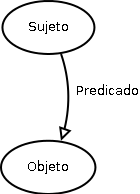
\includegraphics[width=0.2\textwidth]{/triple.png} 
    \caption{Esquema de tripla}
    \label{fig:triple}
  \end{center}
\end{figure}

Usando este modelo se permite la mezcla de datos estructurados y
semi-estructurados a través de diferentes aplicaciones. 

Esta estructura de enlaces forma grafos etiquetados y dirigidos donde los
arcos representan el tipo de relación entre dos recursos, representados por
nodos del grafo (véase figura \ref{fig:triplejena}). 

\begin{figure}[!h]
  \begin{center}
    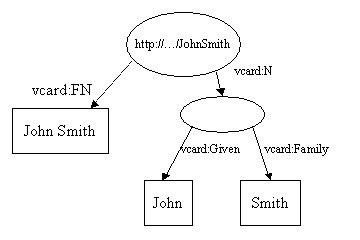
\includegraphics[width=0.6\textwidth]{/triple-jena.png} 
    \caption{Grafo basado en triplas. Extraído de \cite{JENA}}
    \label{fig:triplejena}
  \end{center}
\end{figure}


\subsubsection{\acf{OWL}}

Según \cite{OWL}, se define \acs{OWL} como un lenguaje de Web Semántica
  diseñado para representar conocimiento enriquecido y complejo acerca de
  conceptos, grupos de conceptos y relaciones entre conceptos. \acs{OWL} es un
  lenguaje computacional basado en la lógica de manera que el conocimiento que
  expresa puede ser explotado por programas de computador.

Los documentos generados según el lenguaje \acs{OWL} se conocen como
\textbf{ontologías}. Las ontologías pueden ser publicadas en la \acs{W3C} o
pueden referise o derivarse de otras ontologías. 

\textit{En el contexto de la computación y ciencias de la información, una
  ontología define un conjunto de primitivas de representación con la que
  modelar un dominio de conocimiento} ~\cite{GRUBER}. La finalidad de las
ontologías es ofrecer un modelo formal acerca de un conjunto de conceptos sobre
el cual poder aplicar razonamiento automático . 

De \acs{OWL} derivan tres sub-lenguajes basados en la capacidad expresiva, tal y como cita \cite{OWL}: 

\begin{enumerate}
\item \textbf{\acs{OWL} Lite}: que da soporte a las necesidades básicas del
  usuario cuando lo que se presente es una representación no tan exhaustiva,
  como por ejemplo, recursos, clasificaciones jerárquicas y restricciones
  simples. 
\item \textbf{\acs{OWL} DL (Description Logics)}: soportando más expresividad
  semántica y garantiza que todas las inferencias puedan ser calculadas en un
  tiempo finito.  
\item \textbf{\acs{OWL} Full}: el grado de expresividad es total, pero no
  asegura que las inferencias puedan ser calculadas en un tiempo finito. 
\end{enumerate}


\subsubsection{\acf{SPARQL}}

\acs{SPARQL} es un lenguaje estándar para la consulta de grafos \acs{RDF}. En
\cite{SPARQL} se puede encontrar toda la información y especificación de la
tecnología. 

Muy similar a \acf{SQL}, es un lenguaje declarativo que permite estructurar las
consultas como patrones de \textit{triplas} sobre los cuales extraer instancias
concretas. 

\subsection{Arquitectura}

Tal y como se puede ver en las figuras \ref{fig:swstack} y \ref{fig:swarch}, la arquitectura de la Web Semántica
se fundamenta sobre los principios de la Web tradicional. Estos principios se
pueden resumir: 

\begin{enumerate}
\item Utilización de \acf{URL} para la localización de recursos
\item Uso de \acf{HTML} para la elaboración de documentos, de modo que sea
  entendible por las personas y procesable por los computadores. 
\item Uso de \acf{HTTP} de comunicación cliente-servidor.
\end{enumerate}

\begin{figure}[!h]
  \begin{center}
    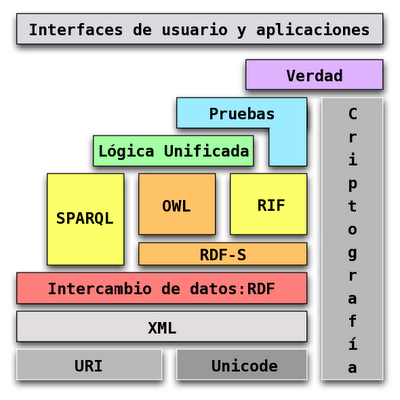
\includegraphics[width=0.6\textwidth]{/sweb-stack.png} 
    \caption{Tecnologías de Web Semántica}
    \label{fig:swstack}
  \end{center}
\end{figure}

Las diferentes capas que se muestran en la figura \ref{fig:swarch} ~\cite{PASTOR} se pueden
definir como :

\begin{itemize}
\item \textbf{Capa de localización y codificación}: el estándar para la
  codificación de caracteres es UNICODE y para la identificación y localización
  de recursos se utilizarán las \acs{URI} o \acs{URL}.
\item \textbf{Capa de sintaxis}: estándares necesarios para la representación de
  información. Cobra especial importancia \acs{XML} puesto que ofrece un formato
  de fácil procesamiento con una sintaxis jerárquica. Como derivación de
  \acs{XML} surge \acs{XML} \textit{namespaces} que habilitará la aparición de
  diferentes vocabularios \acs{XML} en un mismo documento. Esto permite la
  reutilización de recursos que previamente ya se hayan definido. 
\item \textbf{Capa de descripción y estructura}: el uso de \acs{RDF} como
  estándar de representación de recursos, propiedades y relaciones, es el
  siguiente gran salto en la Web Semántica. Al tener una representación de la
  semántica formal, se consigue la interoperabilidad semántica entre
  aplicaciones heterogéneas. 
\item \textbf{Capa de integración lógica de ontologías y reglas de inferencia}:
  estrechamente vinculada con la capa de descripción y estructura, en esta capa se
  amplía la definición de clases, relaciones y propiedades entre recursos,
  utilizando para ello el lenguaje específico \acs{OWL}.
\item \textbf{Capa de consulta}: los recursos ya representados junto con sus
  relaciones ya conforman un hito. A continuación se requiere establecer unos
  mecanismos para búsqueda de triplas. \acs{SPARQL} cumplirá la función de motor
  de búsqueda declarativo sobre archivos \acs{RDF}. 

\end{itemize}


\begin{figure}[!h]
  \begin{center}
    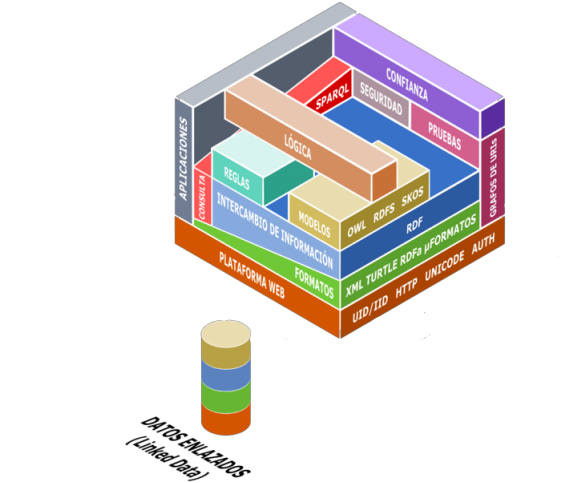
\includegraphics[width=1.0\textwidth]{/sw-archpastor.png} 
    \caption{Arquitectura de la Web Semántica. Extraído de \cite{PASTOR}}
    \label{fig:swarch}
  \end{center}
\end{figure}

\subsection{Ontologías}
\label{sbs:ontologia}

Las ontologías pueden jugar un papel crucial para permitir el procesamiento del
conocimiento, el intercambio y la reutilización basada en la Web entre
aplicaciones. Las ontologías ofrecen una comprensión común de conceptos, con el
fin de que la comunicación entre personas y aplicaciones sea homogénea
\cite{decker_semantic_2000}. 

\subsubsection{Definiciones de ontologías}

\cite{GRUBER} define las ontologías como \textit{una especificación explícita de
  una conceptualización}, refiriéndose este término al modelo abstracto de una
realidad concreta. 

En \cite{studer_knowledge_1998} se profundiza en los términos que engloba la
definición de ontología:

Una ontología es una especificación formal y explícita de una
   conceptualización compartida, donde:
 \begin{itemize}
 \item el término ``conceptualización'' se
   refiere a un modelo abstracto de algún fenómeno en el mundo, identificando
   los conceptos relevantes del mismo,
\item ``explícita'' porque los tipos de
   conceptos utilizados así como las constantes en su uso están explícitamente
   definidas,
\item ``formal'' se refiere al hecho de que la ontología debe ser
   legible para las computadoras, lo que excluye al lenguaje
   natural, y
\item  ``compartida'' refleja la noción de que una ontología captura el
   conocimiento consensuado, es decir, no es privativo para ningún individuo,
   sino que es aceptado por un grupo.

 \end{itemize}


Luego una ontología es una jerarquía que define una serie de clases, atributos y
relaciones para describir un dominio sobre un concepto en concreto cuya
finalidad es servir de herramienta para la representación del conocimiento. 


\subsubsection{Componentes de una ontología}

En \cite{PASTOR} se enumeran los distintos componentes de las ontologías: 

\begin{itemize}
\item \textbf{Clases}: conceptos generales acerca de un determinado dominio. La
  idea básica que se pretende formalizar. 
\item \textbf{Relaciones}: enlace entre conceptos (clases) de un mismo
  dominio.
\item \textbf{Atributos}: representan la estructura del concepto. 
  \begin{itemize}
  \item \textbf{Funciones}: identifican un elemento mediante el cálculo de una
    función. 
  \end{itemize}
\item \textbf{Instancias}: representa un individuo concreto perteneciente a una
  clase. 
\item \textbf{Axiomas}: expresiones siempre ciertas sobre relaciones. 
\end{itemize}


\subsubsection{Clasificación de las ontologías}

A su vez, dependiendo del objetivo de la ontología, se pueden clasificar en
distintos ámbitos tal y como propone \cite{guarino_formal_1998} (véase figura \ref{fig:guarino-taxonto}): 

\begin{itemize}
\item Ontologías de alto nivel (\textit{Top-level ontologies}): describen conceptos muy generales que son
  independientes de un problema particular, tales como espacio, tiempo, objeto,
  evento o acción. 
\item Ontologías de dominio y tarea (\textit{Domain ontologies and task ontologies}): describen respectivamente,
  el vocabulario relacionado con un dominio genérico o con una tarea genérica o
  actividad, especializando los términos de la ontología de alto nivel.
\item Ontologías de aplicación (\textit{Application ontologies}): describen conceptos dependiendo tanto del
  dominio particular como de la tarea, es decir, es una especialización que
  generalmente particulariza \textit{ambos} tipos de ontología. Generalmente
  corresponde con \textit{roles} desempeñados por entidades de dominio mientras
  desarrollan alguna tarea.  
\end{itemize}
 

\begin{figure}[!h]
  \begin{center}
    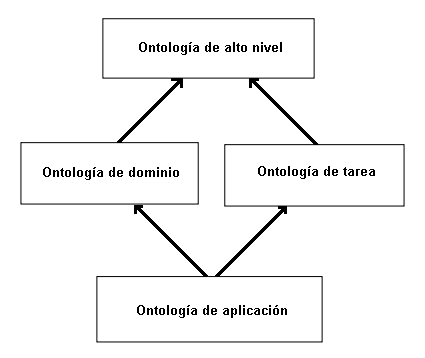
\includegraphics[width=0.6\textwidth]{/ontology-classification.png} 
    \caption{Clasificación de Ontologías. Extraído de \cite{guarino_formal_1998}}
    \label{fig:guarino-taxonto}
  \end{center}
\end{figure}

\subsubsection{Metodología para desarrollo de una ontología en entornos de Web Semántica}

Finalmente, \cite{noy_ontology_2001} propone una secuencia de tareas que todo
desarrollo de cualquier ontología debería incluir: 

\begin{enumerate}
\item Definir las clases en la ontología
\item Organizar dichas clases según una taxonomía
\item Definir propiedades de las clases y los valores que se asocian a esas
  propiedades
\item Completar los valores de las propiedades para cada una de las instancias. 
\end{enumerate}


\subsection{Vocabularios}

Como complemento al concepto de ontología, se describe a continuación el término
vocabulario, frecuentemente usado en gran parte de la bibliografía. 

\subsubsection{Definición}

En la Web Semántica, tal y como se explica en \cite{W3CSW}, los vocabularios definen los conceptos y relaciones usados
para describir y representar un área de conocimiento y así clasificar los
términos en una aplicación particular caracterizando relaciones y
restricciones. Los vocabularios en la práctica pueden ser enormemente complejos
o muy simples (llegando a describir únicamente uno o dos conceptos). 

Según esta definición no queda claro en qué se diferencia un vocabulario de una
ontología, pues realmente no existe una división clara entre estos dos
conceptos. La tendencia es utilizar el término ``ontología'' para una colección
de términos más compleja y formal, mientras que ``vocabulario'' se usa cuando la
flexibilidad en el formalismo no implica necesariamente una pérdida de
significado \cite{W3CSW}. 

Por lo tanto, la función de un vocabulario es similar a la de una ontología en
términos de objetivo final: establecer una representación formal de un
determinado concepto. 

\subsubsection{Ejemplos de vocabulario}

Existen numerosos vocabularios en uso actualmente. A continuación se citan
algunos ejemplos:

\begin{definitionlist}
\item[\acf{DOAP}] 
  El objetivo de este vocabulario es la descripción de proyectos software. Para
  ello, incluye toda la termonología referente al proyecto (licencia, versión de
  producto, dirección de repositorio, \ldots). 
\item[\acf{SKOS}]
 Este vocabulario tiene por objetivo la representación y estructuración de
 esquemas conceptuales tales como taxonomías, esquemas de clasificación o
 tesauros. 

\item[\acf{FOAF}]
  Quizá uno de los más
  extendidos sea \acf{FOAF} \cite{FOAF}. Su finalidad es describir personas,
  relaciones entre ellas así como aspectos de su actividad. Esta tecnología está
  en alza debido a su extensión en las redes sociales. \acs{FOAF} a día de hoy es
  la base de un número considerable de esfuerzo en lo que se conoce como
  movimiento ``open social'', que tratan de facilitar al usuario integrar su
  propia información a través de aplicaciones sociales a través de la Web
  \cite{Allemang:2008:SWW:1386668}. 

  \acs{FOAF} trabaja según el principio de \acf{AAA}. En el caso de \acs{FOAF} los
  temas usualmente son otras personas ~\cite{Allemang:2008:SWW:1386668}. 

  En la figura \ref{fig:foaf} y en el listado \ref{code:foaf} pueden verse ejemplos de uso de este vocabulario. En
  la figura se aprecian dos recursos (\texttt{foaf:ian} y \texttt{foaf:mary}), dos
  propiedades (\texttt{foaf:knows} y \texttt{foaf:firstName}) y un literal
  (``\texttt{Mary}''). En el listado \ref{code:foaf} se expone un documento
  describiendo algunas entidades y relaciones. 

\end{definitionlist}




\begin{figure}[!h]
  \begin{center}
    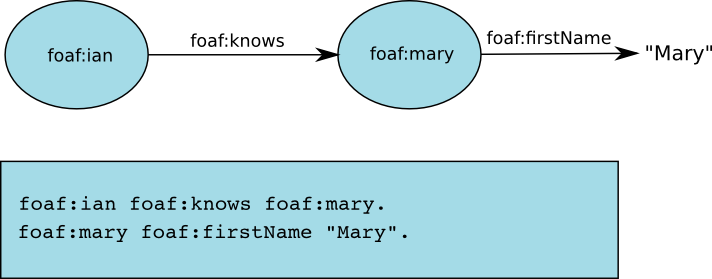
\includegraphics[width=0.8\textwidth]{/foaf.png} 
    \caption{Ejemplo de \acs{FOAF}. Extraído de \cite{JENA}}
    \label{fig:foaf}
  \end{center}
\end{figure}

\begin{listing}[
    float=ht,
    language = XML, 
    numbers=left,
    numberstyle=\tiny,
    stepnumber=1,
    numbersep=5pt,
    frame=single,
    caption = {Ejemplo de \acs{FOAF}}, 
    label = code:foaf]
<rdf:RDF
  xmlns:rdf=''http://www.w3.org/1999/02/22-rdf-syntax-ns#''
  xmlns:rdfs=''http://www.w3.org/200/01/rdf-schema#''
  xmlns:foaf=''http://xmlns.com/foaf/0.1/''>

  <foaf:Person>
    <foaf:name>Raul Reguillo Carmona</foaf:name>
    <foaf:title>Mr</foaf:title>
    <foaf:nick>Radulfr</foaf:nick>
    <foaf:weblog rdf:resource=''http://geeklandtryp.blogspot.com.es />
    <foaf:knows>
      <foaf:Person>
        <foaf:name>Ismael Caballero</foaf:name>
      </foaf:Person>
    </foaf:knows>
  </foaf:Person>
</rdf:RDF>

\end{listing}

\subsection{Frameworks para el desarrollo de aplicaciónes de Web Semántica}

En \cite{W3CTools} se puede consultar una lista con todos los frameworks de Web
Semántica disponibles hasta la fecha. En este apartado, se van a nombrar
solamente algunos de ellos por ser especialmente significativos. 

\subsubsection{Apache Jena}
\label{sec:eajena}

Jena es un framework para la construcción de aplicaciones que utilizan
tecnologías semánticas y Linked Data \cite{JENA}. 

En la arquitectura de Jena (véase figura \ref{fig:jenarquitectura}) se pueden encontrar tres bloques diferenciados en función de
las herramientas que engloban: 


\begin{itemize}
\item \textbf{RDF}
  \begin{itemize}
  \item Jena ofrece una \acs{API} para el tratamiento con grafos \acs{RDF},
    serializando las triplas y tratando con ellas de manera ágil y eficiente. 
  \item Paralelamente ofrece un motor \acs{SPARQL} para las consultas sobre los
    archivos semánticos. 
  \end{itemize}
\item \textbf{Triple Store}
  \begin{itemize}
  \item Para hacer persistentes los datos, Jena ofrece \acf{TDB}: una base de
    datos de triplas nativa de alto rendimiento y alineada con el resto de
    tecnologías de Jena. 
  \item Por otra parte, Jena ofrece \textbf{Fuseki} como \textit{endpoint}, es
    decir, como servidor de triplas accesible a través de \acs{HTTP},
    integrándose a la perfección con \acs{TDB}.\label{sbs:fuseki}
  \end{itemize}

\item \textbf{OWL}
  \begin{itemize}
  \item Para trabajar con modelos y \acs{OWL}, Jena propone una \acs{API} específica
    orientada a ontologías. 
  \item Jena igualmente propone una \acs{API} para facilitar el razonamiento y
    comprobar el contenido de los archivos semánticos. Permite especificar
    distintos razonadores. 
  \end{itemize}
\end{itemize}


\begin{figure}[!h]
  \begin{center}
    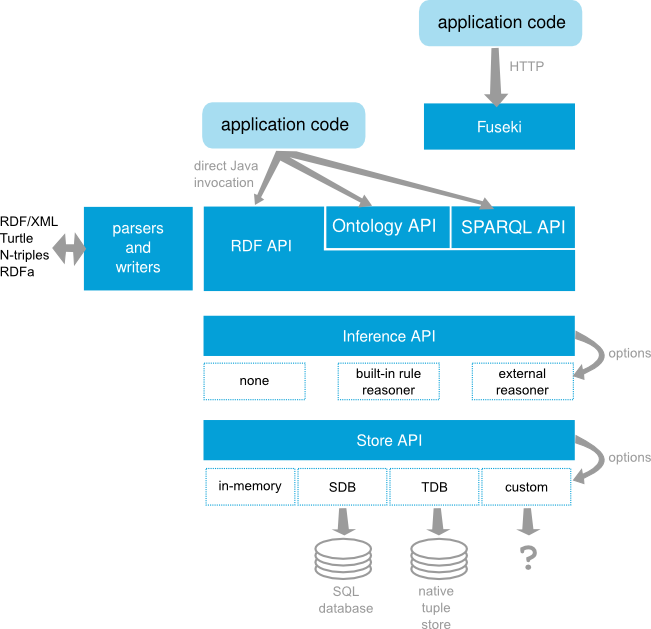
\includegraphics[width=1.0\textwidth]{/jenarqu.png} 
    \caption{Diagrama de la arquitectura de Jena. Extraída de \cite{JENA}}
    \label{fig:jenarquitectura}
  \end{center}
\end{figure}



A continuación se van a definir algunos de los conceptos que maneja Jena así
como se va a introducir brevemente el ámbito de la inferencia en este
framework. 

\begin{definitionlist}
  \item[Modelo]

    A la hora de trabajar con triplas, jena utiliza los llamados
    \textbf{modelos}. Un modelo de Jena es un conjunto de triplas \acs{RDF} con
    el que se puede trabajar de diversas formas: bien para hacer consultas sobre
    él o para aplicar inferencia. Estos modelos son la piedra angular de la
    tecnología puesto que son la fuente del resto de operaciones que se
    desarrollan en este framework. 

  \item[Inferencia]
    La inferencia es un proceso abstracto de derivación de información adicional
    partiendo de los datos \cite{JENA}. De esta manera se utilizará la
    inferencia para hacer explícita información que aparece de forma implícita
    en los datos. 

    La inferencia en Jena consta de dos partes fundamentales: 
    \begin{itemize}
    \item \textbf{Razonadores}: encargados de llevar a cabo la inferencia,
      pudiendo encontrar en Jena los siguientes \cite{JENA}: 
      \begin{enumerate}
      \item Razonador transitivo: ofrece soporte para el razonamiento a través
        de los conceptos de clase y propiedad. Únicamente afecta a propiedades
        transitivas y reflexivas de \texttt{rdfs:subPropertyOf} y
        \texttt{rdfs:subClassOf}. 
      \item Razonador de reglas RDFS: Implementando un subconjunto configurable
        de vínculos RDFS. 
      \item Razonadores para OWL, OWL Mini, OWL Micro: Un conjunto no completo
        para la implementación de inferencia basada en OWL/Lite y OWL/Full. 
      \item Razonador de reglas genéricas: Se basa en reglas definidas, mediante
        el encadenamiento hacia adelante, hacia atrás e híbrido. 
      \end{enumerate}
    \item \textbf{Reglas}: las reglas son sentencias usadas para aplicar inferencia en un
      determinado modelo. Jena implementa un lenguaje propio para la edición de
      estas reglas. 
    \end{itemize}

Se puede consultar un esquema del razonamiento en Jena en la figura
\ref{fig:jenareasoning}. 

\begin{figure}[!h]
  \begin{center}
    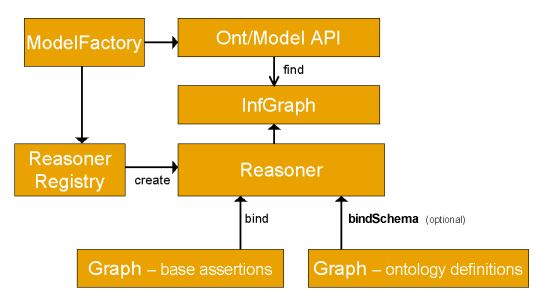
\includegraphics[width=1.0\textwidth]{/reasoner-overview.png} 
    \caption{Razonamiento en Jena. Extraída de \cite{JENA}}
    \label{fig:jenareasoning}
  \end{center}
\end{figure}


\end{definitionlist}

\subsubsection{Sesame}

OpenRDF Sesame es un framework estándar \textit{de-facto} para el procesado de
datos RDF \cite{OPENRDF}. Sesame incluye operaciones para el procesamiento,
consulta, almacenamiento e inferencia sobre \acs{RDF}. Al igual que Jena, Sesame
contiene un número considerable de herramientas para la construcción de
aplicaciones de tecnologías semánticas. 


\subsubsection{CubicWeb}

CubicWeb \cite{CUBIC} es otro framework, \textit{open source}, para la realización de
aplicaciones semánticas. Está escrito en Python. Sus características engloban:

\begin{itemize}
\item Soporta \acs{OWL} y \acs{RDF}
\item \acf{RQL}
\item Herramientas de migración para desarrollo ágil
\item Una librería de \textit{cubes} como pequeños módulos al estilo de Ruby. 
\end{itemize}

\subsubsection{Comparativa}


En el cuadro \ref{tab:comparativa} se pueden contemplar algunas características de los
frameworks anotados anteriormente, pudiendo encontrarse una relación más
completa en \cite{W3CTools}: 


\begin{table}[hp]
  \centering
  {\small
  % Comparativa

\begin{tabular}{|p{.2\textwidth}|p{.2\textwidth}|p{.2\textwidth}|p{.2\textwidth}|}
  \tabheadformat
  \tabhead{Framework}         &
  \tabhead{Lenguaje}          &
  \tabhead{Licencia}          &
  \tabhead{Versión}           \\
\hline
Apache Jena         & Java   & Apache License 2.0 & 3.4.0 / July 17, 2017 \\
\hline
Sesame              & Java   & BSD-style license  & 2.8.9 / January 26, 2016     \\
\hline
CubicWeb            & Python & Lesser General Public License  & 3.19.1 / June 3, 2014     \\
\hline
\end{tabular}



% Local variables:
%   coding: utf-8
%   ispell-local-dictionary: "castellano8"
%   TeX-master: "main.tex"
% End:

  }
  \caption[Comparativa de frameworks de Web Semántica. Extraída de \cite{W3CTools}]
  {Comparativa de frameworks de Web Semántica. Extraída de \cite{W3CTools}}
  \label{tab:comparativa}
\end{table}



\section{\acf{LD}}

En esta sección se incluyen los conceptos clave respecto de los principales
movimientos de datos abiertos y datos enlazados. 

\subsection{Definición de \acs{LD}}

Berners-Lee en \cite{bernerslee:2009} enfatiza la publicación de los datos en la
Web no únicamente como exposición de los mismos, sino mediante el establecimiento de enlaces
de forma que personas o máquinas puedan explorar una Web de datos. De esta
manera se pueden encontrar datos relacionados. 

La mayor parte del contenido en la Web está construido con documentos. Estos
documentos a su vez tienen enlaces hacia otros documentos cuyo contenido puede
estar o no formalizado. El movimiento \acs{LD} pretende dar un paso más allá,
estableciendo relaciones entre los datos de manera global (véase figura \ref{fig:dbpedialod}). Para ello, \acs{RDF}
y las \acs{URI} toman un papel crucial. \cite{bernerslee:2009} expone
sus cuatro reglas para \acs{LD}:  

\begin{enumerate}
\item Usar \acs{URI} como nombres para los conceptos.
\item Usar \acs{HTTP} para que las personas puedan acceder a esos nombres. 
\item Proporcionar información útil cuando la \acs{URI} sea desreferenciada,
  usando estándares como \acs{RDF} o \acs{SPARQL}. 
\item Incluir enlaces a otras \acs{URI}, de manera que los usuarios puedan
  descubrir nuevos conceptos. 
\end{enumerate}


\begin{figure}[!h]
  \begin{center}
    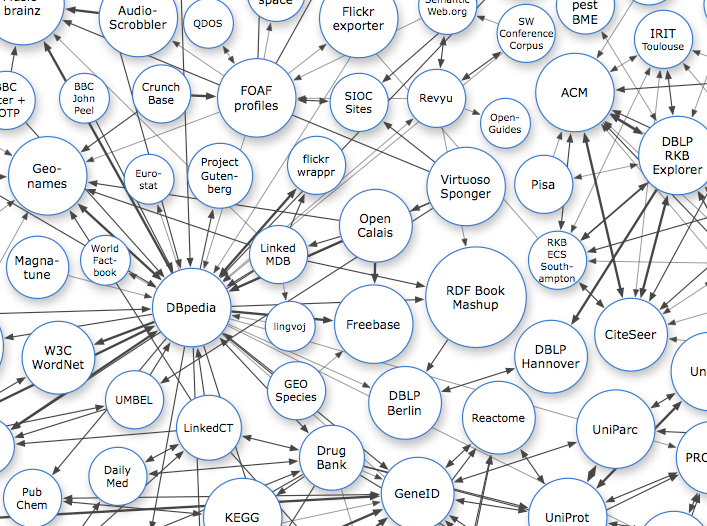
\includegraphics[width=1.0\textwidth]{/lod.png} 
    \caption{Esquema \acs{LD} DBpedia}
    \label{fig:dbpedialod}
  \end{center}
\end{figure}



\cite{bizer_linked_2009} establece a su vez una serie de pasos básicos para la
publicación de \acs{LD}: 

\begin{enumerate}
\item Asignar \acs{URI} a las entidades descritas por el conjunto de datos y
  proveer el desreferenciado de las \acs{URI} a través del protocolo \acs{HTTP}
  en representaciones de \acs{RDF}.
\item Establecer enlaces \acs{RDF} a otros recursos de datos en la Web, de tal
  manera que los usuarios puedan navegar a través de la Web de los datos
  siguiendo enlaces \acs{RDF}.
\item Facilitar metadatos sobre los datos publicados, de manera que los usuarios
  puedan evaluar la calidad de los datos publicados y escoger entre diferentes
  medios de acceso.
\end{enumerate}

Aprovechando \acs{LD} la información en la Web Semántica puede verse desde
diferentes niveles de granularidad, desde el grafo universal formado por todos
los documentos \acs{RDF} en la Web, pasando por documentos individuales hasta
sus triplas \cite{ding_tracking_2005} (véase figura \ref{fig:rdfmol}). 


\begin{figure}[!h]
  \begin{center}
    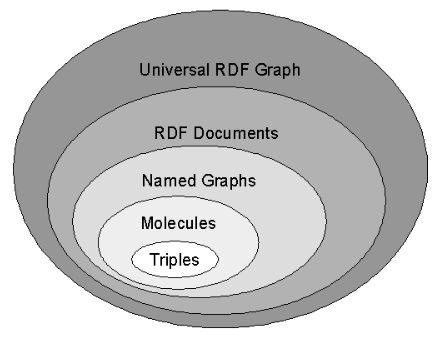
\includegraphics[width=0.6\textwidth]{/rdfmol.png} 
    \caption{Niveles de granularidad en la Web Semántica. Extraído de \cite{ding_tracking_2005}}
    \label{fig:rdfmol}
  \end{center}
\end{figure}


\subsection{\acf{OD} y \acf{LOD}}

Por otra parte los \acf{OD}, se presentan en ausencia de
formatos privativos, información pública y reutilizables procedentes de
organizaciones tales como las gubernamentales. Así, \acf{LOD} serán todos
aquellos datos enlazados que sean abiertos. \cite{bernerslee:2009} define
\acs{LOD} como \acs{LD} que es liberado bajo licencia abierta que no impida su
reuso de manera gratuita. 

Asimismo, define las cinco estrellas de calidad de \acs{LOD}: 

\begin{itemize}
\item \textbf{$\star$} Los datos están disponibles en la Web, independientemente del
  formato, pero con licencia abierta, para que sean \acs{OD}.
\item \textbf{$\star \star$} Disponible para la lectura por parte de máquinas, es decir,
  datos estructurados. Por ejemplo, utilizar una tabla Excel en lugar de una
  imagen escaneada de dicha tabla. 
\item \textbf{$\star \star \star$} Como el anterior, pero en formato no propietario. En
  este caso formato \acf{CSV} en lugar de Excel.
\item \textbf{$\star \star \star \star$} Todo lo anterior y además, usar estándares
  abiertos de \acs{W3C} (\acs{RDF} y \acs{SPARQL}) para identificar conceptos,
  de manera que otros usuarios puedan apuntar a este contenido. 
\item \textbf{$\star \star \star \star \star$} Lo anterior y además, enlazar estos datos
  a los de otros usuarios para proporcionar un contexto. 
\end{itemize}

\subsection{\acs{LOD} en la actualidad}

Empresas del sector privado y público se han dado cuenta de las ventajas que
\acs{OD} y \acs{LOD} pueden ofrecerles. Es por ello que están surgiendo muchas
aplicaciones tanto a nivel nacional, donde estos movimientos aún no están
demasiado extendidos, como a nivel internacional. En \cite{APPS} se encuentra
una lista con una serie de aplicaciones realizadas utilizando tecnología
\acs{OD} y \acs{LOD}. A continuación se exponen algunos ejemplos. 


\subsubsection{Bus Guru}

\textbf{Bus Guru} es una aplicación para iOS que monitoriza en tiempo real la
situación de los autobuses urbanos así como su hora de llegada estimada para una
parada (véase figura \ref{fig:busguruapp}). 

\subsubsection{Bus Gijón}

Igualmente en el ámbito nacional, existen aplicaciones que aprovechan los datos
abiertos generados en tiempo real por dispositivos empotrados en autobuses y
marquesinas. Un caso homólogo a \textbf{Bus Gurú} es \textbf{Bus Gijón} (figura \ref{fig:busgijon}), que
recaba información del portal de \acs{OD} \url{https://datos.gijon.es} para
obtener información de los autobuses. 


\begin{figure}[!h]
  \begin{center}
    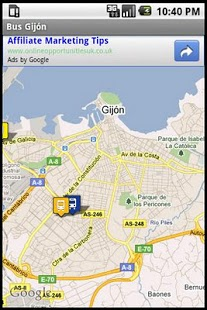
\includegraphics[width=0.3\textwidth]{/busgijon.jpg} 
    \caption{Bus Gijón App}
    \label{fig:busgijon}
  \end{center}
\end{figure}


\begin{figure}[!h]
  \begin{center}
    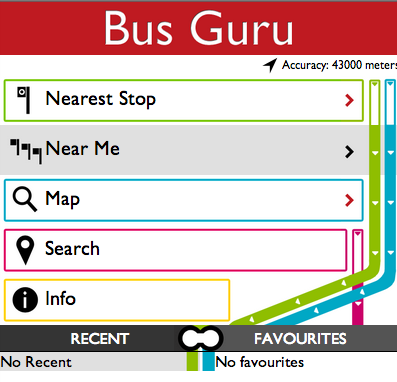
\includegraphics[width=0.3\textwidth]{/busguru.png} 
    \caption{Bus Gurú App}
    \label{fig:busguruapp}
  \end{center}
\end{figure}




\section{Calidad de Datos}
\label{sec:dqREF}


En ~\cite{Strong:1997:DQC:253769.253804} se identifican tres roles a
la hora de tratar los datos: 

\begin{enumerate}
\item \textit{Data producers}: aquellas entidades encargadas de \textbf{generar}
  los datos. 
\item \textit{Data custodians}: personas responsables del \textbf{almacenamiento
  y procesado} de los datos. 
\item \textit{Data consumers}: personas o grupos que \textbf{usan} los datos. 
\end{enumerate}


Debido a que los
diferentes roles tendrán concepciones distintas de lo que los datos significan
para ellos según su papel en un sistema, pueden encontrarse distintas
perspectivas de lo que significa calidad de datos. Dos de las
principales perspectivas son \textit{Meeting Requirements} y \textit{Fitness for
  Use}. 

\begin{itemize}
\item{\textit{Meeting requirements} \cite{BPM}: Los datos tienen calidad si
  satisfacen los requisitos que fueron establecidos. Los \textbf{requisitos
    de datos} que son especificados, por ejemplo, con un modelo \acf{ER} en el
  que se subrayan cómo se van a relacionar los datos como conjunto, es decir, un
  marco arquitectónico para los datos. En \cite{conf/ekaw/FurberH10} y
  \cite{Furber:2011:TVD:1966901.1966903} se pueden consultar aproximaciones a la
  calidad de datos desde este punto de vista.}

\item{\textit{Fitness for use} \cite{Strong:1997:DQC:253769.253804}: Se dice que
  los datos tienen calidad si son válidos para el propósito por el que son
  requeridos, es decir, considerando la calidad de los datos en el
  \textbf{contexto} de uso. En \cite{conf/webist/CaballeroVCP08} se adopta esta
  aproximación.}


\end{itemize}


\subsection{Dimensiones de Calidad de Datos}

La perspectiva \textit{Fitness for Use} se centra en los \textit{Data consumers},
considerando datos de alta calidad aquéllos que son apropiados al usuario final
en el contexto de uso. Debido a ello, se deben considerar aspectos tales como
\textit{utilidad} o \textit{usabilidad} y en definitiva, todo aquel aspecto que
pueda repercutir en la experiencia del usuario. 

Puesto que la calidad de los datos dependerá del propósito, se requiere
considerar una serie de \textbf{categorías}. La calidad de datos es un concepto
que es necesario evaluar desde distintos criterios o \textbf{dimensiones} (\acf{DQD})
~\cite{Strong:1997:DQC:253769.253804}. Al conjunto de dimensiones de calidad de
datos utilizados para evaluar un conjunto de datos se le conoce como
\textbf{Modelo de Calidad de Datos}. En el cuadro \ref{tab:DQD} se detallan
conjuntos de dimensiones de calidad agrupadas por categorías. 


\begin{table}[!h]
  \centering
  {\small
  % Data Quality Dimensions

\begin{tabular}{|p{.4\textwidth}|p{.4\textwidth}|}
  \tabheadformat
  \tabhead{Categoría de Calidad de Datos}         &
  \tabhead{Dimensiones de Calidad de Datos}       \\
\hline
Intrínseca         & Precisión, Objetividad, Credibilidad, Reputación \\
\hline
Accesibilidad      & Accesibilidad, Acceso seguro \\
\hline
Contextual         & Relevancia, Valor añadido, Temporalidad, Completitud,
Cantidad de datos adecuada \\
\hline
Representacional   & Interpretabilidad, Facilidad de entendimiento,
Representación concisa, Representación consistente \\
\hline
\end{tabular}



% Local variables:
%   coding: utf-8
%   ispell-local-dictionary: "castellano8"
%   TeX-master: "main.tex"
% End:

  }
  \caption[Categorías y dimensiones de \acs{DQ}]
  {Categorías y dimensiones de \acs{DQ}. Extraído de \cite{Strong:1997:DQC:253769.253804}}
  \label{tab:DQD}
\end{table}


Pese a que existan modelos de calidad de datos consistentes, la calidad de datos
no deja de ser un concepto subjetivo, puesto que para un mismo conjunto de
datos se pueden obtener niveles de calidad radicalmente distintos dependiendo del
usuario o el rol que haga uso de ellos, incluso sobre la misma dimensión de
calidad ~\cite{Wang:1998:PPT:269012.269022}. 

A continuación se detallarán algunas dimensiones de calidad de datos. 

\subsection{Completeness}
\label{sbs:completeness}

Dentro de todas las posibles dimensiones de calidad, existen subconjuntos que
cobran especial relevancia. \textit{Completeness} es, por norma general para
todos los autores, una dimensión de obligada presencia en todos los trabajos. 

Dentro de esta dimensión, en la bibliografía se proponen distintas métricas que
contemplan el concepto de \textit{completitud} desde diversas perspectivas. Como
se comprobará en adelante (véase Sección \ref{sec:dqassessment-completeness}), en el presente trabajo se ha optado por una única
visión, más compacta, sencilla y acorde a lo que un usuario puede esperar acerca
de la presencia de valores no nulos en Linked Data.

\subsubsection{Definición}

\cite{zaveri_quality_2013} define \textbf{Completeness} como el grado en el que toda la información
requerida está presente en un conjunto de datos particular. En general, esta
definición se puede extender sobre otros factores tales como profundidad de los
datos, anchura y alcance para la tarea que se quiera realizar. 

\cite{pipino_data_2002} amplía esta definición. Define Completeness como el
grado en que los datos no han desaparecido y poseen la suficiente amplitud y
profundidad para la tarea en cuestión. 

Por otro lado, la norma \acs{ISO} 25012 (véase \cite{citeulike:5717734}) define Completeness como el grado en el que
los datos asociados con una entidad tienen valores para todos los atributos
esperados e instancias relacionadas en un contexto de uso específico. 


\subsection{Accesibility}
\label{sbs:accessibility}

En entornos de Web Semántica y Linked Data tiene especial importancia el hecho
de que dichos datos sean de fácil acceso. La palabra \textit{accesiblidad}
cuando se habla de datos enlazados cobra un valor mayor que en otras
dimensiones. Es preciso que los datos enlazados estén, en efecto, adecuadamente
enlazados. 

\subsubsection{Definición} 


\acs{ISO} 25012 (véase \cite{citeulike:5717734}) define \textit{Accessibility} como el grado en el que los datos
puedan ser accedidos en un contexto de uso específico, particularmente por gente
 que necesite tecnología de apoyo o una configuración especial debido a alguna
 discapacidad. 

Por otra parte \cite{pipino_data_2002} define Accessibility como el
grado en que los datos están disponibles y son accesibles fácil y rápidamente. 


\section{Calidad de Datos en \acs{LD}}
\label{sec:lddq}

Actualmente, existen autores tales como \cite{zaveri_quality_2013} o
\cite{Furber:2011:TVD:1966901.1966903} que comienzan a aplicar conceptos de
\acs{LD} para algunas dimensiones de calidad. Para ilustrarlo, se muestran
algunas métricas propuestas en estos trabajos para las \acs{DQD} Completeness y
Accessibility. 

\subsubsection{Métricas para Completeness}
\label{sec:dqassessment-completeness}
\label{metricasdq}

\cite{zaveri_quality_2013} propone una serie de métricas para la evaluación de
esta dimensión. 

\label{schemacompleteness}
\label{interlinking}
\begin{enumerate}
\item \textit{Schema Completeness}: grado en el que las clases y propiedades de
  una ontología están representadas. También conocido como \textit{ontology
    completeness}.

\item \textit{Property Completeness}: evaluación sobre los valores perdidos de
  una propiedad específica.

\item \textit{Population Completeness}: siendo el porcentaje de todos los
  objetos del mundo real de un determinado tipo que están representados en los
  conjuntos de datos. 

\item \textit{Interlinking completeness}: refiriéndose al grado en el que las
  instancias en el conjunto de datos están interconectadas. Esta métrica consta
  de especial importancia en Linked Data. No obstante esta métrica concreta
  puede entenderse (como así se abordará en este trabajo, en la Sección \ref{sec:dqassessment-accessibility}) como una
  particularización de otra dimensión de calidad bien distinta:
  \textit{Accesibility}. 

\end{enumerate}

\cite{conf/ekaw/FurberH10} ofrece un conjunto de consultas
\acs{SPARQL} que permiten identificar problemas de integración de calidad de
datos. Se pueden comprobar dos ejemplos en los listados
\ref{code:query1} y \ref{code:query2} extraídos de ese mismo trabajo. 



\begin{listing}[
  float=ht,
  language = SQL,
  numbers=left,
  numberstyle=\tiny,
  stepnumber=1,
  numbersep=5pt,
  frame=single,
  caption  = {Consulta \acs{SPARQL} para identificación de literales perdidos (I)},
  label    = code:query1]
SELECT ?s 
WHERE { {
  ?s a <class1> .
  ?s <prop1> "". }
UNION{
  ?s a <class1> .
  NOT EXISTS {
  ?s prop1> ?value}}}

\end{listing}



\begin{listing}[
  float=ht,
  language = SQL,
  numbers=left,
  numberstyle=\tiny,
  stepnumber=1,
  numbersep=5pt,
  frame=single,
  caption  = {Consulta \acs{SPARQL} para identificación de literales perdidos (y
  II)},
  label    = code:query2]
SELECT ?s 
WHERE { {
      ?s a <class1> .
      ?s <prop1> <value1>.
   NOT EXISTS{
      ?s <prop2> ?value2 .
   }
   }UNION{
      ?s <prop1> <value1> .
      ?s <prop2> "".
   }}
\end{listing}



\subsubsection{Métricas para Accessibility}
\label{sec:dqassessment-accessibility}
\cite{zaveri_quality_2013} considera Accessibility como una
categoría que a su vez contiene cuatro dimensiones, cada una con sus métricas: 

\begin{itemize}
\item \textbf{Disponibilidad}: grado en el la información está presente y
  preparada para su uso. Sus métricas propuestas son: 
  \begin{itemize}
  \item \textit{Accessibility of the server}: comprobación sobre el servidor
    \acs{SPARQL} ante una consulta.
  \item \textit{Accessibility of the \acs{SPARQL} endpoint}:  comprobación sobre el servidor
    \acs{SPARQL} ante una consulta.
  \item \textit{Accessibility of the \acs{RDF} dumps}: comprobación sobre la
    recuperación de datos en un contenedor de datos \acs{RDF}.
  \item \textit{Dereferencability issues}: comprobación en el momento que una \acs{URI}
    devuelva un error del código de respuesta o enlace roto. 
  \item \textit{No structured data available}: detección de enlace caído o
    cuando una \acs{URI} sin metadatos \acs{RDF} o sin redirección, devuelva el
    código de error pertinente. 
  \item \textit{Misreported content types}: detección de si el contenido es
    susceptible a ser consumido y si el contenido puede ser accedido. 
  \item \textit{No dereferenced back-links}: detección de todos los enlaces
    propios al conjunto de datos: localmente disponibles. 
  \end{itemize}
\item \textbf{Rendimiento}: Eficiencia del sistema vinculado al conjunto de
  datos de manera que cuanto más eficiente sea la fuente de datos, un sistema
  puede procesar más eficientemente los datos. Las métricas para esta dimensión
  son: 
  \begin{itemize}
  \item \textit{No usage of slash-\acs{URI}s}: uso de \acs{URI}s abreviadas
    cuando existen grandes cantidades de datos. 
  \item \textit{Low latency}: si una petición \acs{HTTP}  es contestada en un
    tiempo medio de un segundo. 
  \item \textit{High throughput}: número de peticiones \acs{HTTP} contestadas
    por segundo. 
  \item \textit{Scalability of a data source}: detección de si el tiempo en
    responder una cantidad de diez peticiones, dividido entre diez, no es mayor
    que el tiempo en responder una petición. 
  \item \textit{No use of prolix \acs{RDF} features}: detección del uso de
    primitivas \acs{RDF} tales como contenedores y colecciones. 
  \end{itemize}
\item \textbf{Seguridad}: Grado en el que los datos pueden ser restringidos y de
  esta manera protegidos contra alteraciones ilegales y uso no permitido. Las
  métricas propuestas son las siguientes:
  \begin{itemize}
  \item \textit{Access to data is secure}: uso para login de credenciales o uso
    de protocolos específicos. 
  \item \textit{Data is of propietary nature}: el propietario de los datos
    permite el acceso únicamente a ciertos usuarios. 
  \end{itemize}
\item \textbf{Tiempo de respuesta}: Medición del retardo, generalmente en
  segundos, entre el envío de una consulta por el usuario y la recepción de los
  resultados. Existe una métrica para esta dimensión:

  \begin{itemize}
  \item \textit{Delay in response time}: retardo entre el tiempo de envío de una
    petición por el usuario y la recepción de dicha petición por el sistema. 
  \end{itemize}

\end{itemize}

\section{Big Data}

\subsection{Concepto}

Desde los comienzos del siglo XXI han tiendo lugar una serie de cambios muy
significativos en la industria de las tecnologías de la información, tales como
el nacimiento del Internet de las Cosas, Computación en la Nube y la aparición
de las Redes Sociales.

El desarrollo y explotación de estas tecnologías ha propiciado que la cantidad
de los datos que se generan por unidad de tiempo se haya incrementado a una
velocidad sin precedentes, trayendo consigo la necesidad de cómputo de tales
volúmenes de información heterogénea, en tiempos razonables y de manera escalable.

\textit{Big Data} es por lo tanto un concepto que surge debido a la necesidad del
uso de herramientas y técnicas específicas para procesar esta información,
imposible para los sistemas transaccionales comunes ~\cite{BARR:que-es-big-data}.


De esta manera, el concepto \textit{Big Data} se
puede caracterizar según la definición de las tres V's:

\begin{itemize}
\item \textbf{Volumen}: en referencia al tamaño del conjunto de datos. No hay un
  número estándar que defina a partir de qué tamaño del conjunto de datos se
  pueda empezar a hablar de Big Data. No obstante, cuando el conjunto de datos
  no es susceptible de ser procesado en un único nodo, y requiere la presencia
  de varios de éstos, puede decirse que es Big Data. Luego el orden de magnitud
  puede ir desde los cientos de GB hasta los Petabytes. 
\item \textbf{Velocidad}: referenciando a las necesidades relativas al consumo o proceso
  de datos en tanto se aproximen al tiempo real (\textit{real time}) o próximos
  al tiempo real (\textit{near real time}).
\item \textbf{Variedad}: en relación ala heterogeneidad de los datos. Esto incluye
  representaciones diversas de datos estructurados, como diversas fuentes
  relacionales, datos semiestructurados o datos no estructurados, como pudieran
  ser imágenes o vídeo. 
\end{itemize}

Adicionalmente se ha extendido esta definición a medida que las tecnologías y la
problemática ha cambiado, encontrando:

\begin{itemize}
\item \textbf{Valor}: considerando el beneficio que se puede extraer de los datos bajo la
  premisa que tanto la complejidad de la extracción del valor, como dicho
  beneficio en sí mismo se incrementa junto con el volumen.
  
\item \textbf{Veracidad}: entendiendo como el grado de confianza que se establece sobre
  los datos. 
\end{itemize}

Cada dimensión deja de manifiesto un problema concreto que hay que afrontar en
un contexto Big Data. No obstante estas definiciones, a medida que las
tecnologías evolucionan, se adaptan y renuevan, pudiendo hablar sobre la
existencia de hasta 9Vs. 


\begin{figure}[!h]
  \begin{center}
    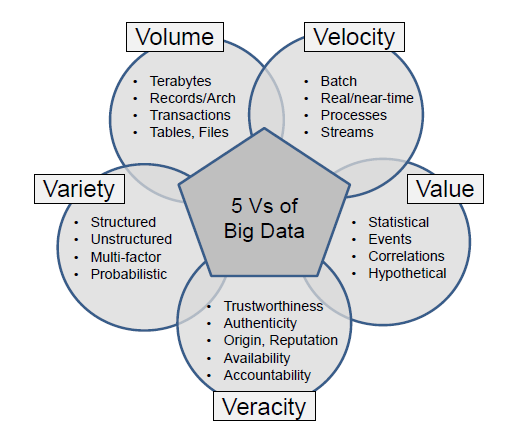
\includegraphics[width=0.5\textwidth]{/5Vs.png} 
    \caption{5vs del Big Data}
    \label{fig:5Vs}
  \end{center}
\end{figure}

En ~\cite{map_reduce} se define por primera vez un modelo de procesamiento y
generación de grandes conjuntos de datos, a través de funciones \textit{map} y
\textit{reduce}, apoyándose en que muchos problemas del mundo real son
expresables en estos términos.

En adelante se desarrollaron multitud de frameworks y herramientas que basándose
en estos principios optimizarán y permitirán el procesado escalable de grandes
volúmenes de información, cumpliendo con el paradigma de las 5Vs. Entre ellos,
se encuentra el ecosistema Hadoop que se describirá con detalle en la sección
\nameref{sec:eco-hadoop}.

\begin{figure}[!h]
  \begin{center}
    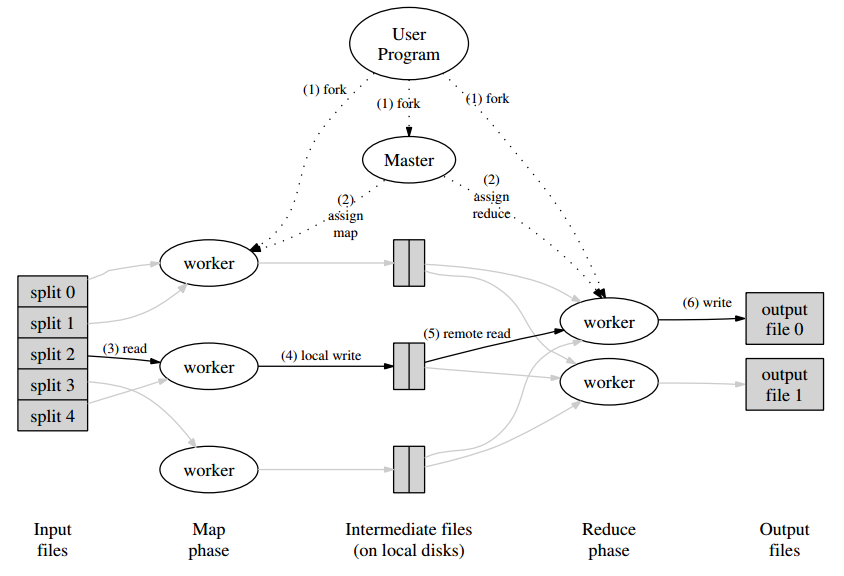
\includegraphics[width=1\textwidth]{/mapred.png} 
    \caption{MapReduce: ejecución ~\cite{map_reduce}}
    \label{fig:mapred}
  \end{center}
\end{figure}


Este modelo consiste en el particionado de los datos de entrada y procesado en
paralelo de dichas particiones por varios nodos, gestionados por un nodo maestro
que ejerce de árbitro y orquestador. En la etapa final, la
unificación de los resultados parciales en torno a una solución final se lleva a
cabo por otro conjunto de nodos que combinarán el resultado en uno o varios
archivos de salida.

Al cierre del 2015, los miembros de la ITU (Unión Internacional de
Telecomunicaciones), aprobaron la primera norma de Big Data, estableciendo la
primera definición oficial ~\cite{ITU}:

\textit{Paradigma para hacer posible la recopilación, el almacenamiento, la
  gestión, el análisis y la visualización, potencialmente en condiciones de
  tiempo real, de grandes conjuntos de datos con características heterogéneas}.

\subsection{Desafíos}

Cuando la volumetría y la disparidad de los datos está presente, existe una
serie de desafíos que deben afrontarse a la hora de acometer un proyecto ~\cite{DBLP:journals/isci/ChenZ14a}:

\begin{itemize}
\item \textbf{Captura y almacenamiento}: debido al ritmo de crecimiento de los
  datos así como a su origen disperso, el modo en el que se acceden, capturan y
  almacenan representa una primera barrera a superar. 
\item \textbf{Descubrimiento y limpieza}: referente a tratamiento de la información previo a
  su procesamiento, análisis exploratorio, gestión de datos perdidos o
  corruptos. 
\item \textbf{Transmisión}: el ancho de banda es un factor limitante cuando se
  habla en un contexto de Big Data y puede representar el cuello de botella de
  un sistema si no se gestiona correctamente el movimiento de tales volúmenes de
  datos.
  
\item \textbf{Análisis y visualización}: llevar a cabo un análisis de volúmenes
  masivos de datos implica desarrollar técnicas tanto a nivel hardware como
  software para permitir dichos análisis. Igualmente la visualización resulta un
  factor crucial a la hora de obtener lecturas fiables de cara a la
  interpretabilidad de dichos datos.
  
\end{itemize}


\subsection{Frameworks}

Existe una gran cantidad de frameworks y ecosistemas dedicados al procesamiento
distribuido de grandes volúmenes de información. Entre ellos caben destacar el
ecosistema Hadoop y las soluciones de Amazon Web Services, que serán descritos a
continuación.


\subsubsection{Ecosistema Apache Hadoop}
\label{sec:eco-hadoop}

El ecosistema Hadoop se ha convertido en el estándar \textit{de facto} a la hora
de llevar a cabo proyectos Big Data. Se organiza a través de una serie de
módulos encargados de diversas operaciones en el contexto de un cluster Big
Data ~\cite{HADOOP-ecosystem}.

Entre sus principales componentes caben destacar los siguientes:

\begin{itemize}
\item \textbf{HDFS}: Hadoop Distributed File System, como sistema de archivos
  distribuido y escalable. 
\item \textbf{Hadoop MapReduce}: framework para escribir aplicaciones que puedan
  procesar grandes volúmenes de información en paralelo en el contexto de un
  cluster, de una manera tolerante a fallos, siguiendo el modelo MapReduce. 
\item \textbf{YARN}: Yet ANother Resource Negotiator es un framework para la
  gestión de recursos de un cluster, encargado de balancear la carga, asignar
  nodos a los distintos trabajos y liberar recursos. 
\item \textbf{Pig}: plataforma de alto nivel para crear programas que se
  ejecutan sobre HDFS, a través de un lenguaje de programación de scripts que
  permiten realizar operaciones ETL (Extract, Transform and Load) sobre datos
  guardados en HDFS. 
\item \textbf{Hive}: proyecto que se ejecuta sobre HDFS con el fin de establecer
  una plataforma de consulta y análisis a través de una interfaz SQL. 
\item \textbf{Oozie}: orquestador de tareas dentro del ecosistema Hadoop. 
\item \textbf{Sqoop}: herramienta para el traspaso eficiente de datos entre HDFS
  y otras soluciones de almacenamiento, tales como bases de datos relacionales o
  ficheros de texto plano. 

\item \textbf{Flume}: solución de recolección y distribución de grandes
  volúmenes de datos entre distintas fuentes.
\item \textbf{HBase}: base de datos distribuida, escalable y no relacional. 
\item \textbf{Zookeeper}: servicio centralizado para el mantenimiento, la
  configuración, nombrado y sincronización de los distintos servicios
  ejecutándose en el contexto de un cluster Hadoop. 
\end{itemize}

Posteriormente se han ido agregando a proyectos apache nuevos frameworks
destinados a cubrir necesidades específicas o a mejorar el rendimiento de los
actuales:

\begin{itemize}
\item \textbf{Spark}: ~\cite{SPARK} es un framework para el procesado de grandes volúmenes de
  información. La ventaja principal respecto de Hadoop MapReduce es que el
  procesamiento se realiza en memoria en lugar de en disco, con lo cual la
  velocidad se incrementa en varios órdenes de magnitud. Se basa en el concepto
  de \acf{RDD} como estructura de datos distribuida básica, asentando sobre ésta
  otras abstracciones como son los Dataframes, que en versiones recientes del
  framework se han convertido en la recomendación de uso. Análogos a los
  Dataframes de lenguajes como R, son estructuras de datos similares a tablas de
  bases de datos relacionales y ofrecen primitivas de consulta similares. Spark
  además tiene como complemento una serie de
  herramientas de alto nivel:
  \begin{itemize}
  \item \textbf{SparkSQL}: módulo para el procesamiento distribuido de datos
    estructurados. Ofrece una interfaz parecida a consultas SQL y mantiene
    información estructural acerca de los datos distribuidos. 
  \item \textbf{MLlib}: librería de machine learning que incluye una serie de
    algoritmos distribuidos, supervisados y no supervisados, pipelines,
    persistencia y utilidades para dar soporte al proceso de aprendizaje
    automático de manera distribuida. 
  \item \textbf{GraphX}: es uno de los componentes más recientes de
    Spark. Incluye una abstracción \textit{Graph} que trabaja directamente sobre los
    dataset distribuidos permitiendo operaciones básicas en el manejo de
    grafos.
  \item \textbf{Spark Streaming}: es una extensión del núcleo de Spark, que
    introduce el concepto de mini-batch como unidad operativa básica y ofrece un
    procesamiento distribuido y tolerante a fallos en streaming. Los datos
    pueden ser ingestados desde distintas fuentes, tales como Kafka, Kinesis o
    sockets TCP. 
  \end{itemize}
\item \textbf{Kafka}: plataforma de streaming distribuida, ideada para dar
  soporte a aplicaciones real-time. 
\item \textbf{Mahout}: framework que ofrece una serie de algoritmos distribuidos
  de Machine Learning. 
\end{itemize}

\subsubsection{Soluciones Amazon Web Services}
\label{sec:eco-aws}

Amazon Web Services es una colección de servicios en la nube, homólogos a los
que se encuentran en el ecosistema Hadoop, que establece una plataforma de
computación.

Entre los principales caben destacar:

\begin{itemize}
\item \textbf{S3}: Simple Storage Service, equivalente a HDFS, ofrece un sistema de archivos
  distribuido, altamente escalable e integrado en los demás servicios. 
\item \textbf{EC2}: Elastic Compute Cloud, ofrece capacidad de cómputo adaptable
  a través de servidores que pueden realizar autoescalado en los centros de
  datos de amazon, versátiles para hospedar sistemas software. 
\item \textbf{EMR}: Ealstic Map Reducec proporciona un marco de Hadoop hospedado que permite
  hospedar datos en instancias EC2 escaladas dinámicamente. 
\item \textbf{Kinesis}: equivalente a Kafka, permite la recopilación,
  procesamiento y el análisis de datos streaming en tiempo real. 
\end{itemize}


\subsection{Datos Semánticos en entornos Big Data}

Si bien los frameworks anteriormente descritos ofrecen un conjunto de
herramientas de procesado de datos de propósito general, no existe a día de hoy
una versión madura de éstos que se haya convertido en un estándar para el
procesado de grandes volúmenes de datos semánticos. Si bien existen un par de
referencias que están comenzando a abrir esta vía: 

\begin{itemize}
\item \textbf{Jena Elephas}: como parte del stack de Jena, Elephas es un
  conjunto de librerías que proveen de herramientas para el procesado de datos
  RDF sobre Hadoop. No obstante el módulo se encuentra actualmente en una fase
  Beta ~\cite{JENE:jena-elephas}. 
\item \textbf{Sansa Stack}: Scalable Semantic Analytics Stack, es un motor de
  procesamiento tolerante a fallos que permite computación distribuida sobre
  datos RDF. Actualmente en la versión 0.2 y en desarrollo ~\cite{SANSA-stack}.
\end{itemize}

